\chapter{Local Correlation Methods (I): Tools and Concepts \label{cha:LOCAL0}}

While computational chemistry has emerged as a reliable experimental tool, the inherent steep scaling of its most accurate methods like coupled cluster or perturbation theory often imposes strict limits on the maximum molecular system size that can be treated. Even the Hartree-Fock method formerly scales with O(N$^4$), and becomes prohibitively expensive for larger molecules if no further approximations are introduced. For post-Hartree-Fock methods, the major bottle necks are the transformation of the 2-electron repulsion integrals from the atomic orbital into the molecular orbital basis, and evaluation of the working equations using these integrals. The $OVOV$-type MO integrals, as they appear in coupled cluster and M{\o}ller-Plesset perturbation theory, are given by
\begin{equation}
\cn{ia}{jb} = \sum^{vir}_b C_{\sigma b} \sum^{vir}_a C_{\nu a} \sum^{occ}_j C_{\lambda j} \sum^{occ}_i C_{\mu i} \cn{\mu\nu}{\lambda\sigma}
\end{equation}
The AO-MO transformation step scales quartically with system size. Over the years, several different strategies have been proposed to speed up this step. Rank-reduction approaches like density fitting or the Cholesky decomposition, split the 4-index integral tensor into a product of two 3-index tensors, which reduces the memory footprint and the \emph{prefactor} of the transformation. Methods that exploit the nearsightedness of the electrons use a different molecular orbital representations, such as local molecular orbitals or natural orbitals, to obtain a more compact representation of the virtual MO space, and consequently reduce the \emph{scaling}. The AO-MO transformation may also be completely skipped by reformulating the working equations in an atomic orbital basis and using sparsity to speed up the calculations.

This chapter introduces the most important tools used in local correlation methods which will be discussed in the next chapter.

\section{Sparsity in Electronic Structure Theory}

Sparsity is a core concept in electronic structure theory. Many of the most commonly encountered matrices and tensors exhibit some form of sparsity, for example, the 2-electron repulsion integrals in the AO basis. This section analyses in detail the different possible types of sparsity.

\FloatBarrier

\subsection{Element-Wise Sparsity of Electron Integrals}

Molecular electron integral evaluation can become prohibitively expensive for large systems, especially the four-dimensional electron-repulsion integral (ERI) tensor which formerly scales as $\ccpx{4}$. It is therefore imperative to exploit the exponential decay of the GTO basis.

Consider a model system consisting of $n$ hydrogen atoms arranged in a line, with a distance of 1 $a_0$ between one another, and a primitive 1s Gaussian function attached to each atom. Figure \ref{fig:HCHAIN_ERINZE} shows the scaling behavior of the overlap and electron repulsion integrals for this toy system. A blue line is used to show the number of total elements, while the green line represents the number of significant integrals with an absolute value below 1e-10. From observing both graphs, it becomes apparent that for increasing number of atoms, many of the electron integrals can be ignored. Therefore, one only needs to store integrals above a certain threshold. This is also known as \emph{element-wise sparsity}.

\begin{figure}[h]
\centering
\begin{subfigure}{0.45\linewidth}
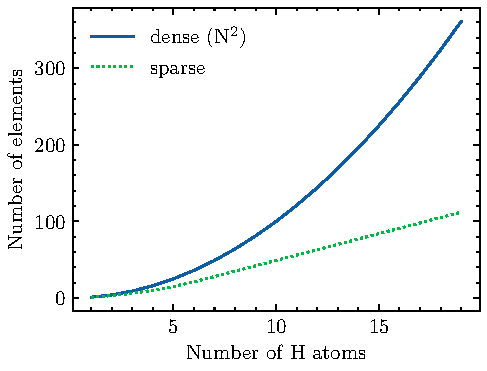
\includegraphics[scale=0.8]{Pics/overlap_nze}
\caption{}
\end{subfigure}
\begin{subfigure}{0.45\linewidth}
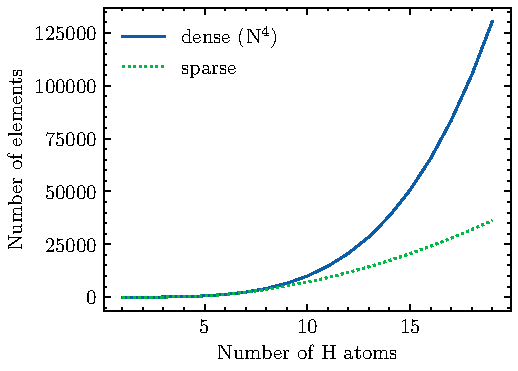
\includegraphics[scale=0.8]{Pics/eri_nze}
\caption{}
\end{subfigure}%
\caption[Sparsity of overlap and electron repulstion integrals]{(a) Number of significant entries (green line) in the overlap matrix for a hydrogen atom chain, with a threshold of 1e-10. The blue line shows the total number of elements for the dense matrix, which scale as $N^2$. (b) Number of significant entries (green line) in the electron repulsion integral tensor for a hydrogen atom chain, with a threshold of 1e-10. The blue line shows the total number of elements for the dense tensor, which scale as $N^4$.}
\label{fig:HCHAIN_ERINZE}
\end{figure}

\begin{figure}
\centering
\begin{subfigure}{0.45\linewidth}
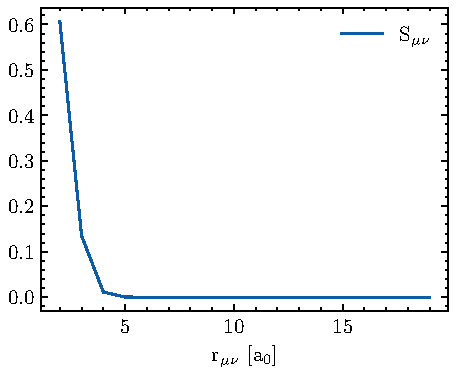
\includegraphics[scale=0.8]{Pics/overlap_decay}
\caption{}
\end{subfigure}
\begin{subfigure}{0.45\linewidth}
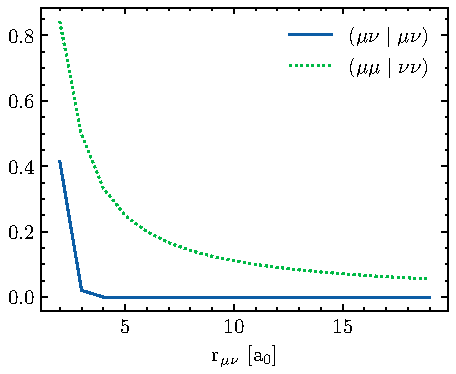
\includegraphics[scale=0.8]{Pics/eri_decay}
\caption{}
\end{subfigure}%
\caption[Decay of the overlap and electron repulsion integrals]{(a) Magnitude of the overlap integral between two Gaussian 1s orbitals as a function of distance $r$ (exponential decay). (b) Magnitude of the electron repulsion integral between two Gaussian 1s orbitals as a function of $r$. The short range interaction $\cn{\mu\nu}{\mu\nu}$ decays at a  much faster rate with $e^{-r^2}$, compared to the long range interaction $\cn{\mu\mu}{\nu\nu}$ with $1/R$.}
\label{fig:HCHAIN_DECAY}
\end{figure}

\subsubsection{Linear Scaling Overlap Integrals}

While the overlap integrals formerly scale with $\ccpx{2}$, it can be shown that the number of significant elements scales \emph{linearly}. First, consider the product of two 1s GTOs $\chi_{A}$ and $\chi_{B}$, centered at $\mathbf{A}$ and $\mathbf{B}$, with exponents $\alpha$ and $\beta$. The Gaussian product theorem (GPT) states that the result is itself also a (scaled) Gaussian function
\begin{equation}
\chi(A,\alpha) \chi(B,\beta) = e^{-\alpha \left\lvert \mathbf{r} - \mathbf{A} \right\rvert^2} e^{-\beta \left\lvert \mathbf{r} - \mathbf{B} \right\rvert^2} = \kappa \chi(P,\alpha+\beta)  
\end{equation}
\noindent with the scaling factor $\kappa$ 
\begin{equation}
\kappa = e^{-\frac{\alpha\beta}{\alpha+\beta}\left\lvert \mathbf{A} - \mathbf{B} \right\rvert^2}
\end{equation}
\noindent and the center-of-charge coordinate $P$
\begin{equation}
\mathbf{P} = \frac{\alpha \mathbf{A} + \beta \mathbf{B}}{\alpha + \beta}
\end{equation}
\noindent Spatial integration yields the expression for the overlap between $\chi_A$ and $\chi_B$
\begin{equation}
S_{AB} = \int \kappa \chi_{P} dr = \kappa \left(\frac{\pi}{\alpha + \beta}\right)^{3/2}
\end{equation} 
\noindent The magnitude of the overlap integral is proportional to the scaling factor $\kappa$ which decays exponentially with the distance between GTO centers. In the case of the model system given above, where $\alpha = \beta$, the distance at which the integral falls below a certain threshold $\eps$ is given by 
\begin{equation}
d_s = \sqrt{\alpha^{-1} ln \left[ \left( \frac{\pi}{2\alpha}\right)^3 \eps^{-1/2} \right]}
\end{equation} 
\noindent Which in our case is equal to 6.9 $a_0$. Each hydrogen atom therefore only has significant overlap with a finite number $n_{max}$ of other centers. For atom chains with $n > n_{max}$, the number of non-zero elements in the overlap matrix will no longer scale as $n^2$, but \emph{linearly} with $n_{max}$. For more realistic, three-dimensional molecular systems, the crossover is less clearly defined due to the non-uniform distribution of atoms and different GTO exponents. Nonetheless, if a system grows sufficiently large, the overlap integrals still scale linearly. Similar arguments can be brought forth for the kinetic-energy integrals as well. 

\subsubsection{Quadratic Scaling Electron Repulsion Integrals} 

Using the Gaussian product theorem established above, we can express the two-electron repulsion integrals of four primitive 1s Gaussian functions $s(A,\alpha)$, $s(B,\beta)$, $s(C,\gamma)$ and $s(D,\delta)$ as
\begin{equation}
\begin{split}
g_{ABCD} &= \int s(A,\alpha) s(B,\beta) \frac{1}{\left\lvert \mathbf{r_1} - \mathbf{r_2} \right\rvert} s(C,\gamma) s(D,\delta) dr \\
&= \int \kappa s(P, \alpha+\beta) \frac{1}{\left\lvert \mathbf{r_1} - \mathbf{r_2} \right\rvert} \lambda s(Q, \gamma+\delta)
\end{split}
\end{equation}
\noindent where $s(P,p)$ and $s(Q,q)$ are Gaussian distributions with
\begin{equation}
\mathbf{P} = \frac{\alpha \mathbf{A} + \beta \mathbf{B}}{\alpha + \beta} ; \quad \mathbf{Q} = \frac{\gamma \mathbf{C} + \delta \mathbf{D}}{\gamma + \delta}
\end{equation}
\begin{equation}
\kappa = e^{-p\left\lvert \mathbf{A} - \mathbf{B} \right\rvert^2} ; \quad \lambda = e^{-q\left\lvert \mathbf{C} - \mathbf{D} \right\rvert^2}
\end{equation}
\begin{equation}
p = \frac{\alpha\beta}{\alpha+\beta}; \quad q = \frac{\gamma\delta}{\gamma+\delta}
\end{equation}

\noindent The coulomb integrals can then be evaluated as 
\begin{equation}
g_{ABCD} = \sqrt{\frac{4 \eta}{\pi}} S_{AB} S_{CD} F_0\left(\eta \left\lvert \mathbf{P} - \mathbf{Q} \right\rvert^2 \right)
\end{equation}
\noindent with the Boys function $F_0$ and the reduced exponent $\eta$ given by
\begin{equation}
\eta = \frac{pq}{p+q}
\end{equation}

\noindent The Boys function is an important function appearing in many expressions for molecular integral evaluation. There are two expressions that bound the Boys function
\begin{equation}
\begin{split}
F_n(x) \leq \frac{1}{2n+1} \quad \textrm{for small } x \\
F_n(x) \leq \frac{(2n-1)!!}{2^{n+1}}\sqrt{\frac{\pi}{x^{2n+1}}} \quad \textrm{for large } x 
\end{split}
\end{equation}
\noindent Using the Boys function's upper bounds, we can derive an upper bound for the electron repulsion integrals of our model system
\begin{equation}
g_{ABCD} \leq min \left\lbrace \sqrt{\frac{4\eta}{\pi}} S_{AB} S_{CD}, \frac{S_{AB} S_{CD}}{\left\lvert \mathbf{P} - \mathbf{Q} \right\rvert} \right\rbrace
\end{equation}
\noindent The left-hand upper bound represents the short-range limit of the Boys function, and the right-hand one the long-range limit. In the short-range limit, i.e. for increasing distance $R_{AB}$ or $R_{CD}$, the magnitude of $g$ decreases \emph{exponentially}. As shown in the previous section, the non-zero elements of the overlap integrals $S_{AB}$ and $S_{CD}$ scale linearly with system size, and therefore the number of significant electron repulsion integrals scales with $N^2$ in total. 
It should be noted, that in the long-range limit with increasing distance $R_{PQ}$ between product densities, the number of elements in $g$ will eventually scale linearly. However, the \emph{algebraic} $1/R$ decay of the long-range interactions is so slow that it practically useless for the size of molecules that can be tackled with current technologies. In the case of the hydrogen atom chain, the integrals $\cn{\mu\mu}{\nu\nu}$ only fall below 1e-10 for $R_{PQ}$ greater than 10$^{10}$ $a_0$. While the long-range decay is impractical for use in the case of the electron repulsion integrals, there are instances such as in atomic orbital MP2 (see Chapter $\ref{cha:LOCAL1}$) where \emph{bra} and \emph{ket} decay as $1/R^4$.
Knowing that the electron repulsion integrals are sparse is only the first step. One also has to develop a \emph{screening} method to avoid computing small integrals, by finding a general upper bound. It has been shown \cite{Roo1951} that $g$ is positive-definite, and fulfills the relationship
\begin{equation}
\sum_{abcd} c_{ab} g_{abcd} c_{cd} > 0
\end{equation}
\noindent where $c$ are one-electron orbital distributions. One can then apply the Schwarz inequality \cite{Hf1989} to obtain an upper bound expression for $g$
\begin{equation}
\cn{\mu\nu}{\sigma\lambda} \leq \cn{\mu\nu}{\mu\nu} \cn{\sigma\lambda}{\sigma\lambda} = Q_{\mu\nu} Q_{\sigma\lambda}
\end{equation}
\noindent The matrix $\mathbb{Q}$ contains the square root of the short-range diagonal entries of $g$, and is also known as the Schwarz matrix. $\mathbf{Q}$ can be evaluated quickly with $\ccpx{2}$ effort and individual integrals can be efficiently screened. It should be noted that Schwarz screening does not take into account the $1/R$ decay between product densities, which makes the method less useful in methods like AO-MP2.

\subsection{Element-Wise Sparsity of the Density Matrix}

The decaying behavior of the density matrix has been extensively studied in solids for atom-centered Bloch and Wannier functions \cite{Koh1959,Ism1999,Goe1994,Goe1998,Tar2002}. It was shown that for insulators, i.e. systems with large band-gaps, the contributions $P_{\mu\nu}$ decay exponentially with increasing distance $R_{\mu\nu}$, while for systems with small or no band gaps, such as metals, the elements decay algebraically. This is also known as Kohn's conjecture \cite{Koh1959}.  
The same observations have been made for non-periodic systems using atomic orbitals as basis. For molecules with a large HOMO-LUMO gap, e.g. alkanes, the number of non-zero elements in the atomic orbital density matrix scales linearly with increasing system size. On the other hand, molecules with strong electron delocalization, such as conjugated polyenes, have have a small HOMO-LUMO gap, and the density matrix elements decay much slower. 
Consider again a chain of hydrogen atoms, equally spaced by $a_0$, each with one 1s Gaussian function, this time with $N_{atom}$ atoms. Figure \ref{fig:HCHAIN_DECAY}a shows the MO diagram for an increasing chain length. In the limit where $N_{atom} \rightarrow \infty$, the system takes on a band structure, similar to how they are encountered in a metal, with a smooth transition between occupied (valence) and virtual (conductance) band. In other words, the HOMO-LUMO gap becomes increasingly small. For a hydrogen chain, where each individual atom contributes one electron, the band is half filled, and the system is a conductor. If the Hydrogen atoms are replaced by Helium atoms, with two electrons per site, the band is fully filled and the system becomes an insulator.
The magnitude of the density matrix elements $P_{\mu\nu}$ is plotted in Figure \ref{fig:HCHAIN_DENSITY}b as a function of increasing distance between 1s functions. The elements decay much slower for the conducting hydrogen chain (algebraic decay), while a rapid exponential decay can be observed in the case of the insulating helium chain. An interesting thing to note is the oscillating values of the density matrix for the hydrogen chain. This phenomenon arises due to the hydrogen atoms pairing up into loosely bound $H_2$ molecules. 

\begin{figure}
\centering
\begin{subfigure}{0.45\linewidth}
\centering
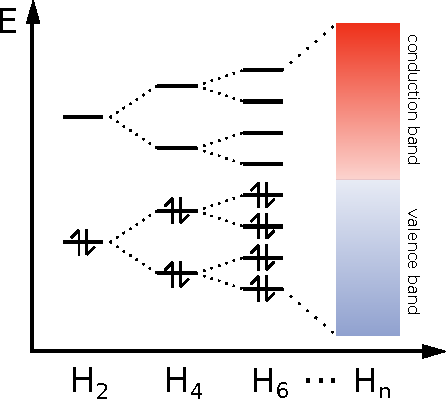
\includegraphics[scale=0.8]{Pics/MOchain}
\caption{}
\end{subfigure}
\begin{subfigure}{0.45\linewidth}
\centering
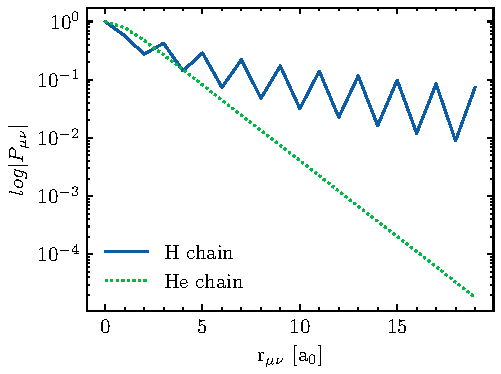
\includegraphics[scale=0.8]{Pics/density_decay}
\caption{}
\end{subfigure}
\caption[MO diagram and decay of density matrix elements in the infinite hydrogen chain]{(a) Molecular orbital diagram for a hydrogen with increasing chain length. (b) Logarithm of the absolute value of the density matrix element $P_{\mu\nu}$ as a function of increasing distance $R_{\mu\nu}$ for a Hydrogen and a Helium atom chain.}
\label{fig:HCHAIN_DENSITY}
\end{figure}


%This sparsity relationship between two AOs is also known as Kohn's conjecture (ref DLMP2).
% exponential decay:
% Koh1959 https://journals.aps.org/pr/abstract/10.1103/PhysRev.115.809
% Ism1999 https://journals.aps.org/prl/abstract/10.1103/PhysRevLett.82.2127
% Goe1994 https://journals.aps.org/prl/pdf/10.1103/PhysRevLett.73.122
% Goe1998 https://journals.aps.org/prb/pdf/10.1103/PhysRevB.58.3501

% algebraic decay
% Tar2002 https://journals.aps.org/prb/abstract/10.1103/PhysRevB.66.233101

\subsection{Diagrammatic Notation}

Hollmann et al. \cite{Hol2017} have introduced a simple graphical representation to show contributing factors to the sparsity of a given matrix, tensor or tensor contraction. Each tensor index is represented as a vertex. Non-connected vertices each contribute $\mathcal{O}(N)$ elements to the overall expression. A sparsity relationship between two indices is represented as an \emph{edge} connecting two vertices. In that case, the number of \emph{pairs} scales as $\mathcal{O}(N)$. Consider the two electron integral tensor $\cn{\mu\nu}{\sigma\lambda}$. From the previous section, we know that the index pairs $\mu,\nu$ and $\lambda,\sigma$ are related by overlap. The diagrammatic representation takes the form:
\begin{center}
\begin{tikzpicture}

\snode{MU}{0,0}{\mu};
\snode{NU}{1,0}{\nu};
\snode{SIG}{2,0}{\sigma};
\snode{LAM}{3,0}{\lambda};

\draw[<->] (MU) -- (NU) node [midway, above] () {S};
\draw[<->] (SIG) -- (LAM) node [midway, above] () {S};

\end{tikzpicture}
\end{center}
\noindent There are two pairs of connected vertices, which indicates that the integrals can be evaluated with $\ccpx{2}$ effort, which is in agreement with the findings above. The $S$ denotes the overlap relationship between vertices.
For another example, consider the Hartree-Fock expression for the exchange matrix
\begin{equation}
K_{\mu\nu} = \cn{\mu\sigma}{\nu\lambda} P_{\lambda\sigma}
\end{equation}
\noindent Diagrammatically, the expression for $\mathbf{K}$ can be represented as
\begin{center}
\begin{tikzpicture}

\snode{MU}{0,0}{\mu};
\snode{NU}{3,0}{\nu};
\snode{SIG}{1,0}{\sigma};
\snode{LAM}{2,0}{\lambda};

\draw[<->] (MU) -- (SIG) node [midway, above] () {S};
\draw[<->] (SIG) -- (LAM) node [midway, above] () {P};
\draw[<->] (LAM) -- (NU) node [midway, above] () {S};

\end{tikzpicture}
\end{center}
\noindent The connection between $\sigma$ and $\lambda$ is also known as a "P-junction" \cite{Nee2009}, which represents the sparsity relationship arising due to the exponential decay of density matrix elements. The sparsity graph is fully connected, which suggests that $\mathbf{K}$ can be evaluated with $\mathcal{O}(N)$ effort. This is indeed the case, as shown by the ONX or LinK method. For linear scaling to emerge, indices of an expression therefore need to be fully linked. This simple but important fact is also known the linked index rule (LIR). Diagrams also show which factors can influence the performance of the scaling, such as diffuseness of the atomic orbitals (slower S decay) or size of of the HOMO-LUMO gap (slower P decay). One can therefore conclude that the expression for $\mathbf{K}$ as given above, is less suitable for large basis sets and conducting systems.

\subsection{Rank Sparsity}

A positive semi-definite matrix $\mathbf{A}$ has the property that it can be decomposed as a product 
\begin{equation}
\mathbf{A} = \mathbf{B} \mathbf{B}^T
\end{equation}
\noindent where $\mathbf{A}$ has dimensions $N$ by $N$, and $\mathbf{B}$ has dimensions $N$ by $rank(A)$. The rank represents the number of linearly independent column vectors in matrix, and for $rank(A) < N$, the matrix is said to  be rank-deficient. The decomposition matrix $\mathbf{B}$ therefore is more compact and needs less storage space than $\mathbf{A}$. There are different ways to compute $\mathbf{B}$, such as Cholesky decomposition or QR decomposition.
The tensor $\cn{\mu\nu}{\sigma\lambda}$ can be represented as a $N_{AO}^2$
by $N_{AO}^2$0 matrix with combined row indices $I = \mu + N_{AO}*\nu$ and column indices $J = \sigma + N_{AO}*\lambda$. Because the tensor has been shown to be positive semi-definite, there also exists a decomposition, such that
\begin{equation}
\cn{\mu\nu}{\sigma\lambda} = A_{(\mu\nu)(\sigma\lambda)} = B_{(\mu\nu)X} B_{(\sigma\lambda)X}
\end{equation}
\noindent The rank of $\mathbf{A}$ is in general much smaller than the combined index range $N_{AO}^2$, and scales linearly rather than quadratically with the number of basis sets. The decomposition tensor $\mathbf{B}$ is therefore 3-dimensional, rather than 4-dimensional, which reduces the storage needed by an order of magnitude from $\ccpx{4}$ to $\ccpx{3}$, ignoring sparsity. In the limit of large molecules, the NZEs of $\mathbf{B}$ also scale with $\ccpx{2}$. Rather than for the molecular integrals in the AO basis, decomposition techniques are more useful for reducing the storage size of molecular integrals in the canonical MO basis
\begin{equation}
\cn{ia}{jb} = C_{\mu i} C_{\sigma a} B_{\mu \sigma X} B_{X \nu \lambda} C_{\nu j} C_{\lambda b} = B_{iaX} B_{Xjb}
\end{equation} 
\noindent The AO-MO transformation step is also drastically sped up, but remains a $\ccpx{4}$ effort. Rank sparsity has therefore little impact on the overall scaling, but rather reduces the scaling \emph{prefactor}. Over the years, different methods have been proposed to compute $\mathbf{C}$, such as density fitting, Cholesky decomposition, pseudo-spectral methods, or tensor hypercontraction.
Density matrices at different levels of theory (Hartree Fock, MP2, CC ...) also exhibit rank sparsity. Decomposition of such matrices play an important role in local molecular orbital schemes and low scaling electronic structure methods, as will be shown in later sections.

% pos def Roo1951 C. C. J. Roothaan, Rev. Mod. Phys., 23, 69 (1951).

% Schwarz inequality Has1989 https://onlinelibrary.wiley.com/doi/abs/10.1002/jcc.540100111

% Good explanation for "linked indices rule" https://aip.scitation.org/doi/pdf/10.1063/1.4926879

% Nee2009 https://reader.elsevier.com/reader/sd/pii/S0301010408005089?token=A38BA6311BBE21191E796ADD75EF1602618F281416BBB8E8C22D61B0C75DF4C02EF402A33375738162D7AA02AFAB8685&originRegion=eu-west-1&originCreation=20210707062425

\FloatBarrier

\section{Density Fitting}

The method of choice in this thesis for the decomposition of two-electron molecular integrals is \emph{density fitting} (DF), also known as \emph{resolution of the identity} (RI). For a brief exploration of other popular methods, the reader is referred to Annex \ref{app:ERIDECOMO}.  

\subsection{Basics of Density Fitting}

The two-electron integrals can be expressed in terms of the charge product densities $\rho_{\mu\nu} = \chi_{\mu} \chi_{\nu}$ as
\begin{equation}
\cn{\mu\nu}{\sigma\lambda} = \int \int \frac{\rho_{\mu\nu}(\mathbf{r_1}) \rho_{\sigma\lambda}(\mathbf{r_2}) }{\mathbf{r_1} - \mathbf{r_2}} d\mathbf{r_1} d\mathbf{r_2}
\end{equation}
The charge densities $\rho$ can be approximated by fitting them to a set of atom-centered auxiliary functions $\chi_P$
\begin{equation}
\rho_{\mu\nu}(\mathbf{r}) = C_{P\mu\nu} \chi_{P}(\mathbf{r}) + \Delta \rho_{\mu\nu}
\end{equation}
\noindent Or in the chemist's notation:
\begin{equation}
\cket{\mu\nu} = C_{P\mu\nu} \cket{P} + \cket{\eps_{\mu\nu}} = \cket{\swtilde{\mu\nu}} + \cket{\eps_{\mu\nu}}
\label{eq:DFAPPROX}
\end{equation}
\noindent where $C_{P\mu\nu}$ are the fitting coefficients, and $\Delta \rho_{\mu\nu}$ or $\cket{\eps_{\mu\nu}}$ is the error introduced by the fitting procedure. Equation \ref{eq:DFAPPROX} is known as the density fitting approximation \cite{Whi1973,Bae1973,Vah1993,Sky2000}. The two-electron integrals then take the form
\begin{equation}
\begin{split}
\cn{\mu\nu}{\sigma\lambda} &= (\swtilde{\mu\nu}|\swtilde{\sigma\lambda}) +  \underbrace{(\swtilde{\mu\nu}|\eps_{\sigma\lambda}) + (\eps_{\mu\nu}|\swtilde{\sigma\lambda})}_\textrm{first order} + \underbrace{\cn{\eps_{\mu\nu}}{\eps_{\sigma\lambda}}}_\textrm{second order} \\
&= (\swtilde{\mu\nu}|\swtilde{\sigma\lambda}) + \eps_J^{(1)} + \eps_J^{(2)} 
\end{split}
\label{eq:DFERROR}
\end{equation}
\noindent Here, $\eps_J^{(1)}$ and $\eps_J^{(2)}$ represent the first order (linear) and second order (quadratic) error. The fitting coefficients are then generally found by minimizing $\eps_J^{(2)}$. Substituting $\scbra{\eps_{\mu\nu}} = \scbra{\mu\nu - \swtilde{\mu\nu}}$ gives
\begin{equation}
\frac{\partial}{\partial C^P_{\mu\nu}} \scn{\mu\nu - \swtilde{\mu\nu}}{\sigma\lambda - \swtilde{\sigma\lambda}} = 0
\end{equation}
\noindent which then yields a set of linear equations
\begin{equation}
\scn{\mu\nu}{P} - \sum_Q C^Q_{\mu\nu} \scn{Q}{P} = 0 
\label{eq:DFLLS}
\end{equation}
\noindent Finding the fitting coefficients by minimizing $\eps_J^{(2)}$ has the important feature that $eps_J^{(1)} = 0$, which can be shown by substituting Equation \ref{eq:DFLLS} back into Equation \ref{eq:DFERROR}. The total electron integral error is therefore \emph{quadratic} in the fitting error. Fitting procedures where the coefficients $C^P_{\mu\nu}$ satisfy Equation \ref{eq:DFLLS} are termed $\emph{robust}$ \cite{Dun2000}. Any restrictions posed on $C^P_{\mu\nu}$ makes $\eps_{1}$ different from zero and the error scales linearly. 
Equation \ref{eq:DFLLS} requires the evaluation of the three-center-two-electron (3c2e) and two-center-two-electron (2c2e) integrals in the auxiliary basis set $\{P\}$
\begin{equation}
\cn{\mu\nu}{P} = \int \int \chi_{\mu}(\mathbf{r_1}) \chi_{\mu}(\mathbf{r_1}) \frac{1}{\mathbf{r_1} - \mathbf{r_2}} \chi_{P}(\mathbf{r_2}) d\mathbf{r_1} d\mathbf{r_2} 
\end{equation}
\begin{equation}
\cn{P}{Q} = \int \int \chi_{P}(\mathbf{r_1}) \frac{1}{\mathbf{r_1} - \mathbf{r_2}} \chi_{Q}(\mathbf{r_2}) d\mathbf{r_1} d\mathbf{r_2} 
\end{equation}
\noindent The fitting coefficients are generally computed by inverting $\cn{P}{Q}$, which leads to the following approximation for the four-center-two-electron integrals (4c2e)
\begin{equation}
\cn{\mu\nu}{\sigma\lambda} \approx \cn{\mu\nu}{P} \cn{P}{Q}^{-1} \cn{Q}{\sigma\lambda}
\end{equation}
\noindent Matrix inversion is a $\ccpx{3}$ computational effort. For more details on precision and best practices involving matrix inversion, see Annex \ref{app:MATINV}.
% Introduced independently by
% (Coulomb) Whi73 https://aip.scitation.org/doi/10.1063/1.1679012
% (Overlap) Bae1973 https://doi.org/10.1016/S0301-0104(99)00271-2 2, 41 (1973).
% Dunlap improved Baerends by using coulomb instead of overlap
% Dun1979 https://aip.scitation.org/doi/pdf/10.1063/1.438728
% Dun1979a https://doi.org/10.1063/1.438313 71, 4993 (1979).
% Begriff "Robust" erstmals hier
% Dun2000 https://www.sciencedirect.com/science/article/pii/S0166128099004339?via%3Dihub

\subsection{Scaling of the 3c2e Integrals}

Using the diagrammatic representation introduced earlier, the 3c2e integral tensor reduces to
\begin{center}
\begin{tikzpicture}
\snode{MU}{0,0}{\mu};
\snode{NU}{1,0}{\nu};
\snode{X}{2,0}{P};
\draw[<->] (MU) -- (NU) node [midway, above] () {S};
\end{tikzpicture}
\end{center}
The number of non-zero elements therefore scales as $\ccpx{2}$, just like for the 4c2e integrals. Similarly, the Schwarz inequality can be used to screen out small integrals
\begin{equation}
\left\lvert \cn{\mu\nu}{P} \right\rvert \leq \left\lvert \cn{\mu\nu}{\mu\nu} \right\rvert^{1/2} \left\lvert \cn{P}{P} \right\rvert^{1/2}
\end{equation}
\noindent As mentioned above, Schwarz screening does not take into account increasing bra-ket distance. The long-range decay is too slow to be of any advantage in the case of the 4c2e integrals. However, it was found \cite{Hol2015} that for an auxiliary density $\chi_P(\mathbf{r}$ with angular momentum $l_P$, the 3c2e integrals actually decay as $1/R^{-1 - l_P}$ with increasing bra-ket distance, establishing a weak but not insignificant sparsity relationship between $\cbra{\mu\nu}$ and $\cket{P}$ 
\begin{center}
\begin{tikzpicture}
\snode{MU}{0,0}{\mu};
\snode{NU}{1,0}{\nu};
\snode{MUNU}{0.5,0}{};
\snode{X}{2,0}{P};
\draw[<->] (MU) -- (NU) node [midway, above] () {S};
\draw[dotted] (MUNU.south) |- (1.25, -0.5) node [below]{$1/R^{-1-l_P}$} -| (X.south);
\end{tikzpicture}
\end{center}
\noindent In principle, the 3c2e integrals can be evaluated with linear effort. Hollmann et al. \cite{Hol2015} have introduced a tight upper bound, known as the SVQl estimator, to exploit this faster decay. Due to the dependence on $l_P$, the screening is most effective with larger basis sets with high angular momentum functions.

The fitting coefficients evaluated as $C^P_{\mu\nu} = \cn{\mu\nu}{Q} \cn{Q}{P}^{-1}$ formerly scale with $\ccpx{3}$
\begin{center}
\begin{tikzpicture}
\snode{MU}{0,0}{\mu};
\snode{NU}{1,0}{\nu};
\snode{Q}{2,0}{Q};
\snode{P}{3,0}{P};
\draw[<->] (MU) -- (NU) node [midway, above] () {S};
\end{tikzpicture}
\end{center}
\noindent due to the inverse of $\cn{P}{Q}$ not being sparse. 

\subsection{Local Density Fitting: Principles} 
The long-range behavior introduced by Equation \ref{eq:DFLLS} is often deemed "unphysical" \cite{Tew2018}. \emph{Local density fitting} (LDF) methods circumvent this problem by forcing a more rapid decay of long-range contributions, either (a) by using a different metric in the fitting procedure or (b) by constructing domains $[\mu\nu]$ that exclude distant fitting functions $P$ a priori. In both cases, Equation \ref{eq:DFLLS} no longer holds and the error in the electron integrals increases linearly with the fitting error. Therefore, the density fitting procedure is no longer robust. Fortunately, LDF methods can use a different expression for the electron integrals which includes the first order terms to remove the linear error
\begin{equation}
\cn{\mu\nu}{\sigma\lambda} \approx (\widetilde{\mu\nu}|\sigma\lambda) + (\mu\nu|\widetilde{\sigma\lambda}) - (\widetilde{\mu\nu}|\widetilde{\sigma\lambda})
\label{eq:DUNLAP}
\end{equation}
\noindent which is known as Dunlap's robust density fitting formula \ref{Dun2000}. It greatly increases accuracy for LDF. 
 
\subsection{LDF (I): Short-Range Metrics}
The first type of LDF methods replaces the fitting procedure in the Coulomb metric in Equation \ref{eq:DFLLS} by a more general expression
\begin{equation}
B_{\mu\nu}^{P} - C_{\mu\nu}^{Q} M_{QP} = 0
\end{equation}  
\noindent where $B_{\mu\nu}^{P}$ and $M_{PQ}$ are the 3c2e and 2c2e integrals given by
\begin{equation}
B_{\mu\nu}^P = \int\int \bfun{\mu}{1}\bfun{\nu}{1} g(\mbf{r_1},\mbf{r_2}) \bfun{P}{2} d\mbf{r_1} d\mbf{r_2}
\end{equation}
\begin{equation}
M_{PQ} = \int\int \bfun{P}{1} g(\mbf{r_1},\mbf{r_2}) \bfun{Q}{2} d\mbf{r_1} d\mbf{r_2}
\end{equation}
\noindent with $g$ being the operator for the local metric. A list of known local metrics is given in Table \ref{tab:DFMETRICS}. Earliest forms of density fitting actually first used an overlap metric to directly minimize the norm of the residual $R_{\mu\nu} = \cbra{\mu\nu} - \cbra{\widetilde{\mu\nu}}$ by the linear least squares methods \cite{Bae1973}, and the fitting coefficients are computed as
\begin{equation}
C^P_{\mu\nu} = S_{PQ}^{-1} (\mu\nu Q)
\label{eq:OVLPMET}
\end{equation}
\noindent where $S_{PQ}$ is the overlap matrix of the auxiliary basis, and $(\mu\nu Q)$ are the 3-center-\textbf{1-electron} overlap integrals. While the overlap metric has the most rapid decay and the quantities in Equation \ref{eq:OVLPMET} can be evaluated in $\mathcal{O}(N)$ time, it has the worst accuracy of all metrics. One solution to this problem is to introduce a metric which is intermediate between overlap and coulomb fitting. Examples include the Yukawa, Coulomb- and Gaussian-attenuated metrics. These intermediate metrics introduce a damping factor $\omega$ to control the sparsity and accuracy of the density fit. In the limit where $\omega \rightarrow 0$, and $\omega \rightarrow \infty$, one recovers the coulomb and overlap metric, respectively. Figure \ref{fig:DFMETRICS} shows the decay behavior of the Coulomb-attenuated metric, for $\omega$ = 0.01, 0.1 and 1.0, compared to the overlap and the Coulomb metric. 

\begin{table}
\centering
\begin{tabular}{cc}
\hline
Metric & $g(r_{12})$ \\ \hline
\multirow{2}{*}{Overlap \cite{Bae1973}} & \multirow{2}{*}{1} \\ & \\
\multirow{3}{*}{Coulomb-Attenuated \cite{Jun2005}} & \multirow{3}{*}{$\dfrac{erfc(\omega r_{12})}{r_{12}}$} \\ & \\ & \\
\multirow{3}{*}{Yukawa \cite{Gil2005}} & \multirow{3}{*}{$\dfrac{e^{-\omega r_{12}}}{r_{12}}$} \\ & \\ & \\
\multirow{3}{*}{Gaussian-Damped \cite{Rei2008}} & \multirow{3}{*}{$\dfrac{e^{-\omega r_{12}^2}}{r_{12}}$} \\ & \\ & \\ \hline
\end{tabular}
\caption{Expressions for the operator $g$ in different local metrics.}
\label{tab:DFMETRICS}
\end{table}

\begin{figure}
\centering
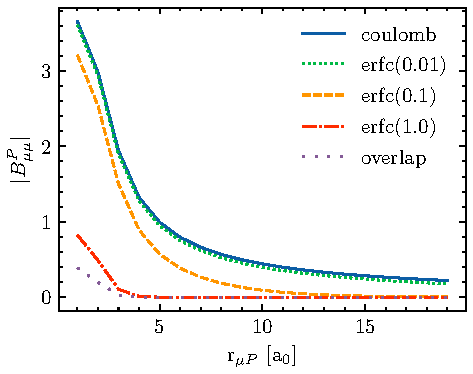
\includegraphics[scale=1.0]{Pics/ldf.pdf}
\caption{Absolute value of the 3c2e integral $B_{\mu\mu P}$ between two 1s GTOs $\mu$ and $P$ with $\alpha$ = 1.0 using different metrics.}
\label{fig:DFMETRICS}
\end{figure}

% A:
% Bae1973 https://www.sciencedirect.com/science/article/pii/030101047380059X?via%3Dihub
% Vah1993 https://www.sciencedirect.com/science/article/pii/0009261493891517?via%3Dihub
% Sky2000 https://www.sciencedirect.com/science/article/pii/S0166128099004340?via%3Dihub
% B: Jun2005 https://www.pnas.org/content/102/19/6692 
% C: Gil2005 https://aip.scitation.org/doi/10.1063/1.2000867 
% D: Rei2008 https://aip.scitation.org/doi/10.1063/1.2956507

% Hol2015 D.S. Hollman, H.F. Schaefer, and E.F. Valeev, J. Chem.Phys.142(2015)

\subsection{LDF (II): Local Domains}

The second method to force locality in density fitting consists in constructing local domains for each atom, pair of atoms or local molecular orbital, and excluding any auxiliary functions that lie outside, which can drastically reduce the dimension of the fitting procedure. 

\subsubsection{Atomic Resolution of the Identity}

The simplest example of a domain is one that includes a single atom. The atomic resolution of the identity (ARI) \cite{Sod2008} uses a fitting procedure where the sum over auxiliary function $Q$ only includes those which are centered on the same atom $A$ as the atomic orbital $\mu$
\begin{equation}
\cket{\widetilde{\mu\nu}} = \sum_{Q \cup A_{\mu}} \cn{P}{Q}_{A_{\mu}}^{-1} \cn{\mu\nu}{Q}
\end{equation}
\noindent Each atom $X$ has its own metric matrix inverse $\cn{P}{Q}_X^{-1}$ which takes the form 
\begin{equation}
\cn{P}{Q}_X^{-1} = B_X \left( \cn{P}{Q}_D + B_X \cn{P}{Q}_{OD}B_X\right)^{-1}B_X
\end{equation}
\noindent where $\cn{P}{Q}_D$ and $\cn{P}{Q}_{OD}$ are the diagonal and off-diagonal part of $\cn{P}{Q}$ respectively. $B_X$ is a so-called \emph{bump matrix} which imposes a fast, but smooth decay between functions $P$ and $Q$ in order to avoid using all functions $P$ for the fitting. For further details, the reader is referred to the original publication. The bump matrix uses multiple distance-dependent criteria which make the ARI less of a black-box method.

% Sod2008 https://aip.scitation.org/doi/pdf/10.1063/1.2828533

\subsubsection{Pair-Atomic Resolution of the Identity}

A more popular and simple variant of atomic density fitting is the pair-atomic resolution of the identity (PARI) method \cite{Mer2013}. As the name implies, the domains include atom \emph{pairs} rather than a single atom. Again expressing it in terms of the fitting procedure
\begin{equation}
\cn{P}{\mu\nu} = \sum_{Q \in A \cup B} \cn{P}{Q} C^Q_{\mu\nu} \quad \forall P \in A \cup B
\end{equation}
\noindent The number of linear equations is equal to the number of non-zero pairs $\mu\nu$, which scales linearly. However, the PARI approach enforces heavy constraints on the fitting coefficients, which leads to large integral errors. Merlot et al. proposed to increase the atomic pair domain with any atoms which lie between A and B. Alternatively, larger and more diffuse basis sets can be used. In both cases, performance is sacrificed for increased accuracy. The absence of any distance dependent parameters or thresholds still make it an attractive method both for Hartree Fock and Post-Hartree Fock methods \cite{Man2015,For2020}.

% Mer2013 https://onlinelibrary.wiley.com/doi/full/10.1002/jcc.23284

\subsubsection{LDF using Local Molecular Orbitals}

Finally, domains can also be formed using local molecular orbitals instead of AOs. LMOs are larger than AOs, but are still generally centered on only a few atoms. The exact atomic sites can be determined for example by using a Mulliken population analysis. Consider the density fitting procedure as proposed by Polly et al. for their LDF-Hartree Fock method \ref{Pol2004}
\begin{equation}
\cn{\mu i}{P} = \sum_{Q \in [i]_{fit}} \cn{P}{Q} C^Q_{\mu i}
\end{equation}
The fitting coefficients are determined individually for each AO-LMO pair $\cket{\mu i}$, and include only those auxiliary functions centered on atoms in the fitting domain $[i]_{fit}$ for which the Mulliken charges are above a given threshold. Although the fitting coefficients need to be recomputed for each update of the MO coefficients, the number of $\cket{\mu i}$ pairs scales linearly with system size. This type of local density fitting and variations thereof are predominantly used in pair-orbital specific local correlation methods, and will be explained in more detail further below. 

% Pol2004 Fast Hartree–Fock theory using local densityfitting approximations

\subsection{LDF (III): Quasi-Robust Density Fitting}

Local density fitting imposes constraints on the fitting procedure, and the integral error consequently scales linearly with the fitting error. Using Dunlap's robust formula is deemed necessary in most cases to achieve acceptable accuracy, but reintroduces the slowly decaying 3c2e integrals. Furthermore, replacing the 4c2e integrals by Equation \ref{eq:DUNLAP} greatly increases the complexity of expressions in electronic structure theory, which is still manageable for ground state methods, but quickly becomes cumbersome for excited states.

Quasi-robust density fitting (QRDF) \cite{Tew2018} aims to combine the exponential decay behavior of LDF with an accuracy comparable to standard density fitting, without the use of Dunlap's formula. Again, consider the fitting procedure 
\begin{equation}
\sum_Q \cn{P}{Q} C^Q_{\mu\nu} = \cn{P}{\mu\nu}
\end{equation}
\noindent The sets of auxiliary functions $\{P\}$ and $\{Q\}$ have different roles. The functions $Q$ fit the charge density $\cket{\mu\nu}$, while the $P$ functions act as \emph{test functions} where the electron integrals should be accurate, i.e. where $\cn{X}{\widetilde{\mu\nu}} \approx \cn{X}{\mu\nu}$. For two functions $\mu$ and $\nu$ not located on the same atom, their charge density $\cket{\mu\nu}$ lies in the vacuum between them, and the atom-centered auxiliary functions may be ill-suited to fit $\cket{\mu\nu}$. For this reason, the fitting procedure draws from all fitting functions $\{P\}$ spanning the whole molecule to cancel out the linear error, which in consequence introduces long-range contributions in $C_{\mu\nu}^P$ in the coulomb metric, even if $\cket{P}$ is not close to $\cket{\mu\nu}$. 
The basic idea of QRDF is to only chose fitting functions $\{P\}$ close to $\cket{\mu\nu}$ via overlap criteria, but still perform the fitting procedure in the coulomb metric.

\subsubsection{The QRDF Fitting Procedure}

For a set of given $\mu,\nu$, select a set of \emph{fitting function} $\{P_{\mu\nu}\} \in \{P\}$ close to $\cket{\mu\nu}$ according to the criteria
\begin{equation}
\left\lvert \sum_R S_{PR}^{-1} (R\mu\nu) \right\rvert > T 
\label{eq:QRDF_FIT}
\end{equation} 
\noindent where $S$ is the auxiliary overlap matrix, and $(R\mu\nu)$ are the 3-center-1-electron overlap integrals. Next, choose a set of test functions $\{Q_{\mu\nu}\} \in \{P\}$ using
\begin{equation}
f(Q_{\mu\nu},P_{\mu\nu}) < R
\label{eq:QRDF_TEST}
\end{equation}
\noindent with
\begin{equation}
f(A,B) = \frac{\alpha \beta}{\alpha + \beta} \left\lvert \mathbf{A} - \mathbf{B} \right\rvert^2
\end{equation}
\noindent where for two auxiliary functions $A$ and $B$, the values $\alpha$, $\beta$ are their smallest primitive exponents and $\mathbf{A}$, $\mathbf{B}$ are their respective positions. The fitting coefficients are then determined via
\begin{equation}
\sum_P \cn{Q_{\mu\nu}}{P_{\mu\nu}} C^P_{\mu\nu} = \cn{Q_{\mu\nu}}{\mu\nu}
\label{eq:QRDFLLS}
\end{equation}
\noindent where the fitting coefficients are accurate within the set of test functions $\{Q_{\mu\nu}\}$. The linear equations in Equation \ref{eq:QRDFLLS} can be solved via QR decomposition or singular value decomposition (SVD) of the rectangular matrix $\cn{Q_{\mu\nu}}{P_{\mu\nu}}$.
The QRDF scheme depends on two parameters, $T$ and $R$. In the limit where $T \rightarrow 0$ and $R \rightarrow \infty$, the standard fitting procedure in the coulomb metric is recovered. 

The fitting functions $\{P_{\mu\nu}\}$ are selected via overlap criteria and therefore scale linearly with the number of pairs $\cket{\mu\nu}$, and consequently the same holds true for the number of test functions $\{Q_{\mu\nu}\}$ close to $\{P_{\mu\nu}\}$ chosen by Equation \ref{eq:QRDF_FIT}. In the limit of large molecules, the size of the rectangular matrix in Equation \ref{eq:QRDF_TEST} becomes constant and the fitting procedure can be evaluated with $\mathcal{O}(N)$ effort. However, a QR decomposition needs to be computed for each set of $\cket{\mu\nu}$, leading to relatively high prefactor which makes the method not competitive for dense 3D structures like water clusters, as will be discussed in the results section.
The QRDF method has been shown to deliver accuracies comparable to standard density fitting, without the use of Dunlap's formula, making it a very attractive alternative to other LDF schemes, especially if one wishes to reduce the complexity of expressions involving LDF.

\subsection{Auxiliary Basis Sets}

The density fitting approximation does not make any assumptions about the size or shape of the auxiliary basis set used. In principle, the fit is exact for the basis set containing all $N_{AO}^2$ Gaussian products $\chi_P = \chi_{\mu} \chi_{\nu}$. In practice, the product space is over-complete and can be represented by much smaller basis sets. Accurate results can be obtained for auxiliary basis sets which are about 4 times larger than the principal basis set they are used with. 

Auxiliary basis sets generally need more higher angular momentum functions than standard basis sets. Consider an isolated, unperturbed atom, with electrons occupying atomic orbitals with highest angular momentum $l_{occ}$. A minimal basis set for this atom contains functions of angular momenta 0 to $l_{occ}$. However, a minimal auxiliary basis set for fitting the product space $\chi_{\mu}^{0...l_{occ}} \chi_{\nu}^{0...\l_{occ}}$ needs functions with maximum angular momentum $2l_{occ}$. For example, 2nd row elements ($l_{occ}$ = 1) need an auxiliary basis set containing d-functions, and first row transition metals ($l_{occ}$ = 2) even need g-functions. Similarly to standard basis sets, to describe atoms in molecules where the orbitals are subject to polarization effects, even higher angular momentum functions are needed to fit polarization functions. In practice, a principal basis set with maximum angular momentum $l_{bas}$ is paired with an auxiliary basis set with highest angular momentum $l_{bas} + l_{occ}$. 

Auxiliary basis sets have the drawback of being method-specific. There are two categories: auxiliary basis sets for density fitted Hartree-Fock (DF-HF) and for density fitted correlated methods (e.g. DF-MP2, DF-CCSD, DF-ADC(2)). Auxiliary basis sets for DF-HF not only need to reproduce Hartree Fock energies, but also need to minimize negative impact on post-Hartree methods. An ill-suited auxiliary basis set leads to a deterioration of the virtual orbital space, and hence an increased error for correlated methods. 

Optimization procedures often try to minimize the energy differences between the standard method and its density fitting approximation in a series of atomic calculations. For example, the jkfit family of basis sets (cc-pVXZ-JKFIT \cite{Wei2002}, def-XVP-JKFIT \cite{Wei2008}) minimize the error
\begin{equation}
\Delta E_{HF} = E_{HF} - E_{DF-HF}
\end{equation}
The RI basis set family (cc-pVXZ-RIFIT \cite{Wei1998}, def2-XVP-RIFIT \cite{Ber1998}) minimizes the same energy difference but for MP2 or Coupled Cluster. 

Another disadvantage of auxiliary basis sets is that the accuracy of the fitting procedure cannot be easily controlled as a function of its composition (number of functions, angular momenta...), but rather extensive benchmarks are needed for each basis set that is introduced. An alternative approach was proposed by Aquilante et al. \cite{Aqu2007} where the fitting basis sets are generated automatically by Cholesky decomposition of the atomic 2-electron integrals
\begin{equation}
\cn{\mu\nu}{\sigma\lambda} = L^X_{\mu\nu} L^X_{\sigma\lambda}
\end{equation}
\noindent The Cholesky vectors $\mathbf{L}_{\mu\nu}$ indicate which product densities should be taken to construct the auxiliary basis. This type of atomic Cholesky decomposition (aCD) basis sets has the advantage that the accuracy can be rigorously controlled by the decomposition threshold $\theta$. To remove linear dependencies in the aCD basis set, another Cholesky decomposition can be performed to yield the atomic compact Cholesky decomposition (acCD) auxiliary basis set \cite{Aqu2009}.

% Dunning JKFIT (1): Wei2002 https://pubs.rsc.org/en/content/articlepdf/2002/cp/b204199p
% Karlsruhe JKFIT (2): Wei2007 https://onlinelibrary.wiley.com/doi/full/10.1002/jcc.20702
% MP2 Karlsruhe Wei1998 https://www.sciencedirect.com/science/article/pii/S0009261498008628
% Dunning (MP2) Ber1998 https://aip.scitation.org/doi/pdf/10.1063/1.476732
% Aqu2007 https://aip.scitation.org/doi/10.1063/1.2777146
% Aqu2009 https://aip.scitation.org/doi/10.1063/1.3116784

\section{Multipole Expansion of the Electron Integrals}

The slow $1/R$ between the product densities $\Omega_{\mu\nu}$ and $\Omega_{\lambda\sigma}$ in the coulomb integrals is a major obstacle for achieving linear scaling in cases where no other sparsity relationship can be established between indices belonging to separate charge densities, e.g. in the evaluation of the coulomb matrix $\mathbf{J}$ versus the exchange matrix $\mathbf{K}$. Luckily, there are approximate methods for integral evaluation that can be computed with $\mathcal{O}(N)$ effort, known as \emph{multipole methods}.

\subsection{Classical and Non-Classical Electron Integrals}

First, consider the concept of classical and non-classical interactions. Two electron integrals are said to be \emph{non-classical} if the two charge densities $\Omega_{\mu\nu}$ and $\Omega_{\sigma\lambda}$ overlap, and \emph{classical} if the charge densities are well separated. In the latter case, the electron integrals represent classical interactions between disjoint point charges, and can be approximated using multipole methods, whereas the non-classical contributions must be evaluated using the more expensive standard integral codes such as McMurchie-Davidson or Obara-Saika. 

Two Gaussian distributions $\Omega_P$ and $\Omega_Q$ are considered \emph{well-separated} up to a target accuracy 10$^{-k}$, if their center-to-center distance $R_{PQ}$ is larger than the sum of their extents $ext_P$ and $ext_Q$:
\begin{equation}
R_{PQ} > ext_P + ext_Q
\end{equation} 
\noindent with the extent of a Gaussian product $P$ defined as 
\begin{equation}
r_P = \frac{1}{\sqrt{p}} erfc^{-1}(10^{-k})
\end{equation}
\noindent where $p$ is the reduced exponent. Another important thing to note is that the number of significant non-classical and classical integrals scale as $\mathcal{O}(N)$ and $\ccpx{2}$ respectively \cite{Hel2000}, which has important consequences as will be shown further below. 

\subsection{Multipole Expansion}

For two well-separated charge distributions $P$ and $Q$, the inverse inter-electronic distance can be expanded in terms of Legendre polynomials $\mathcal{P}$ as
\begin{equation}
\frac{1}{r_{12}} = \sum_{l=0}^{\infty} \frac{\Delta r_{12}^l}{R_{PQ}^l} \mathcal{P}_{l} cos \theta
\label{eq:PARTIALWAVE}
\end{equation}
\noindent with 
\begin{equation}
cos \theta = \frac{\Delta \mathbf{r}_{12}^l \mathcal{R}_{QP}}{\Delta r_{12} R_{QP}} 
\end{equation}
\begin{equation}
\Delta \mathbf{r}_{12} = \mathbf{r}_{1P} \mathbf{r}_{2Q}
\end{equation}
\noindent where $\mathbf{r}_{1P}$ and $\mathbf{r}_{2Q}$ are the distance between electron 1,2 and the centers $P$,$Q$. Equation \ref{eq:PARTIALWAVE} is also known as the partial-wave expansion of the coulomb operator \cite{Arf2012}. Plugging Equation \ref{eq:PARTIALWAVE} into the expression for the two-electron repulsion integrals gives the bipolar multipole expansion of the two-electron integrals
\begin{equation}
g_{abcd} = \sum_{l=0}^{\infty} \sum_{m=-l}^l \sum_{j=0}^{\infty} \sum_{k=-j}^{j} M_{ab}^{lm}(P) T_{lm,jk} M_{cd}^{jk}
\end{equation}
\noindent where $\mathbf{M}_{ab}^{lm}(P)$ is the multipole moment of the charge distribution $P$ with total moment $l+k$, and $\mathbf{T}$ is the so-called interaction matrix. As such, the complicated 6-dimensional evaluation of $g$ can be simply substituted by two 3-dimensional integrations of the multipole moments $\mathbf{M}$ at a much lower cost. For the lowest order expansion, where $l$ = $m$ = 0, and $j$ = $k$ = 0, the multipole moments and the interaction matrix become 
\begin{equation}
M_{ab}^{00} = S_{ab}
\end{equation}
\begin{equation}
M_{cd}^{00} = S_{cd}
\end{equation}
\begin{equation}
T_{00,00} = 1/R_{PQ}
\end{equation}
\noindent The zero order term of the multipole expansion therefore takes the form
\begin{equation}
g_{abcd} \approx \frac{S_{ab}S_{cd}}{R_{PQ}}
\end{equation}

\subsection{Fast Multipole Method}

While the number of individual non-zero integrals still scales with $\ccpx{2}$, the total contribution of all pair-wise interactions to the total energy (Hartree Fock, MP2 ...), can actually be evaluated in $\mathcal{O}(N)$.

For the sake of simplicity, consider a system with point-charge particles with charge $Z$, in a 2-dimensional plane. The total interaction energy is given by
\begin{equation}
U = \sum_{i>j} \frac{Z_i Z_j}{r_{ij}}
\label{eq:INTERENERGY}
\end{equation}
\noindent Evaluating Equation \ref{eq:INTERENERGY} as is takes a quadratic effort. In a first approximation, one can divide the plane into a grid of blocks of equal size, where each block contains a certain number of particles (Figure \ref{fig:FMM1}). Consider the interaction of a single particle $i$ in its source block $C$ with the other particles in the system. The interaction has two contributions: near-field (NF) contributions $U_{NF}$ from the other particles in the source block, and the blocks immediately surrounding it, and far-field (FF) contributions $U_{FF}$ from boxes that are well-separated from $C$. The NF interactions are evaluated directly by summing over all particles $j$ in the near-field
\begin{equation}
U^{NF}_i = \sum_{j \in NF} \frac{Z_i Z_j}{R_{ij}}
\end{equation}
\noindent while FF interactions are computed using multipole expansions $\mathbf{q}_{iC}$ and $\mathbf{q}_A$ of the FF boxes and the particle $i$
\begin{equation}
U^{FF}_i = \sum_{A \in FF} \mathbf{q}_{iC} \mathbf{T}_{CA} \mathbf{q}_A
\end{equation}
\noindent While evaluating the interaction energy at block-level rather than particle-level can considerably reduce the prefactor, the cost of this \emph{single-level multipole method} is still quadratic, since for each particle $i$, there is a system-dependent number of FF boxes. The granularity of the blocks is the same, independent of how far away the blocks are. To achieve linear scaling, the crucial point to realize is that, the further one gets from the source block $C$, the smaller the single-particle interaction $U_i$ becomes, and the less accurately it actually needs to be evaluated. This means that the farther one moves away from C, the larger the FF boxes can be. For this reason, \emph{multi-level multipole methods} introduce a hierarchy of boxes (Figure \ref{FMM2}), where at level 0, the whole system is in a single box, and for each subsequent level, the field is divided into fourths. FF boxes that are closest to C are evaluated at the highest level/granularity $S$. The region of FF boxes surrounding the closest FF boxes are then treated at a lower level $S-1$, and so on, until all interactions have been computed. Because the multipole expansion is evaluated for increasing box size, it can be shown that the total number of boxes is constant for a single particle $i$. This is the basic idea on which the \emph{Fast Multipole Method} (FMM) operates \cite{Gre1987,Gre1994,Din1992}, and it has quickly become one of the most important algorithms in scientific computing, as the problem of particle-particle interaction is not limited to the field of quantum chemistry. FMM can evaluate the total interaction energy $U$ with linear computational complexity.

\begin{figure}
\centering
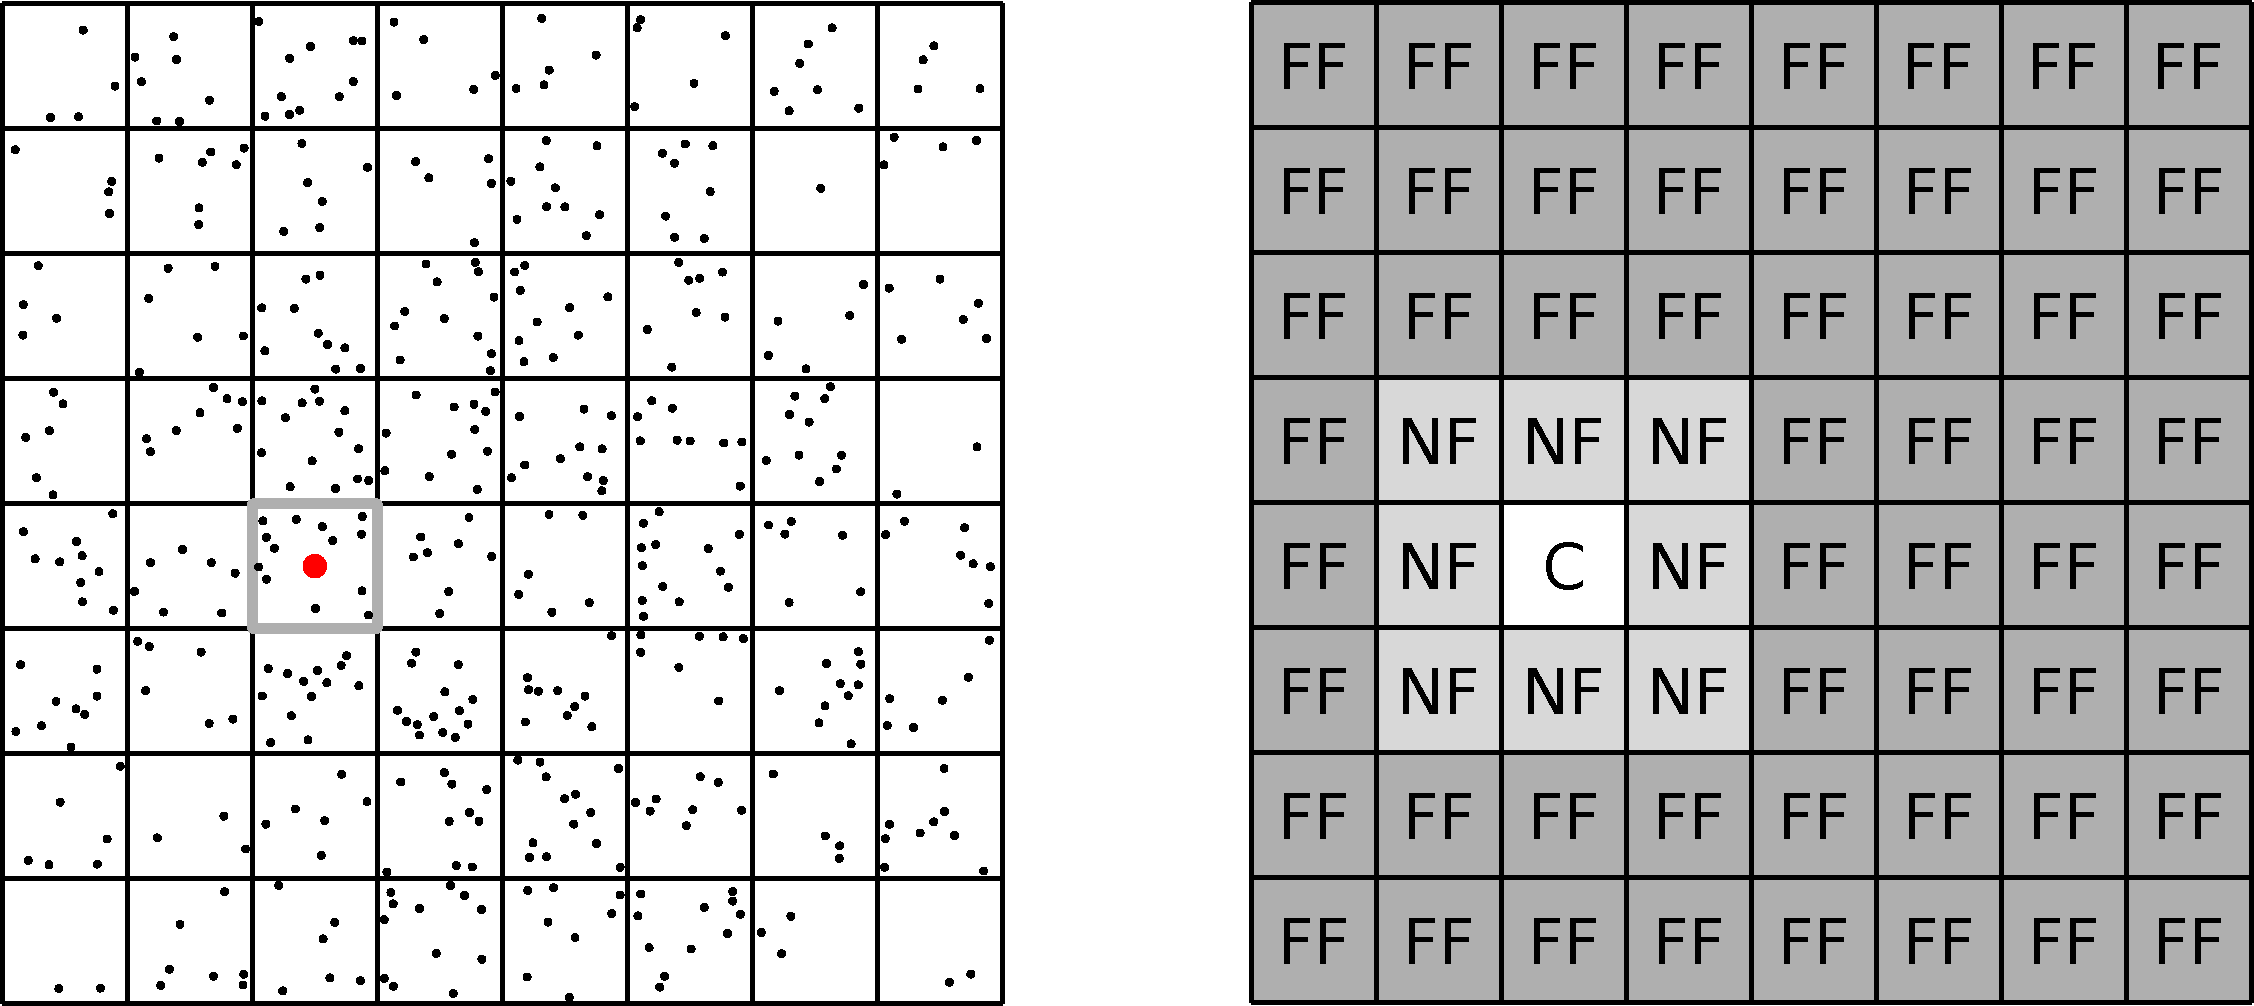
\includegraphics[scale=0.35]{Pics/FMM1}
\caption[Single-level multipole method]{In multipole methods, the system is subdivided into blocks of equal size containing one or more particles. For a reference block $C$, its surrounding blocks are categorized into near-field and far-field contributions which are treated using separate methods.}
\label{fig:FMM1}
\end{figure}

\begin{figure}
\centering
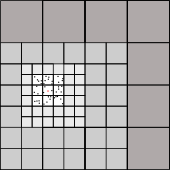
\includegraphics[scale=0.35]{Pics/FMM2}
\caption[Fast multipole method]{In the fast multiple method, the granularity of the boxes becomes coarser the further away they are from the source blocks.}
\label{fig:FMM2}
\end{figure}

% Ark1970 https://www.sciencedirect.com/book/9780123846549/mathematical-methods-for-physicists
% Gre1987 L. Greengard and V. I. Rokhlin, J. Comput. Phys. 73, 325 (1987)
% Gre1994 L. Greengard, Science 265, 909, (1994)
% Din1992 H. Q. Ding, etc.... look at 28, 29 p. 426 big book

\subsection{Continuous Fast Multipole Method}

The fast multipole method does not work for continuous charge distributions like Gaussian functions, as their extents can be quite different from one another, making the separation into NF and FF contributions more difficult. Nonetheless, FMM has been generalized to the continuous case, known as the continuous fast multipole method (CFMM) \cite{Whi1996}. The principle is the same as in multi-level multipole methods, only special care needs to be taken to only include classical contributions into the FMM treatment. For further details, the reader is referred to the original publication. 

\section{The ABCs of LMOs and NOs: Orbital Representations \label{sec:ABCLMO}}

To solve the Hartree-Fock equations in a computationally efficient way, it is favorable to choose the set of molecular orbitals such that they diagonalize the Fock matrix $\mbf{F}$. In other words, they are eigenfunctions of the Fock operator
\begin{equation}
\hat{f}\sket{\phi_i} = \eps_i \sket{\phi_i}
\end{equation} 
\noindent Here, $\{\phi_i\}$ are also known as the \emph{canonical molecular orbitals}. CMOs are not unique in the sense that there are infinitely many alternative molecular representations which yield the same electron density $\mathbf{P}$. Quantities like the total wave function energy or the electronic density are said to be \emph{orbitally invariant}. Non-observables like the MO energies are not preserved under orbital rotation. Let $\mbf{C}$ be the CMO coefficient matrix. A new solution to the HF equations can then be generated by applying a unitary transformation such that
\begin{equation}
C^{new}_{\mu \olj} = U_{ji} C_{\mu i} \qquad \mbf{UU}\pdg = \mbf{1}
\end{equation} 
\noindent There are different reasons why one would want to use another MO basis: they can (a) offer a more intuitive picture for the interpretation of chemical phenomena and (b) help to achieve are more localized and compact representation of the wave function which is helpful for local correlation methods.

There are two significant types of molecular representations besides CMOs: local molecular orbitals (LMOs) and natural orbitals (NOs). The following sections will introduce both  types in more detail.

\subsection{Local Molecular Orbitals}

In contrast to canonical molecular orbitals, which are generally delocalized over the whole molecule, local molecular orbitals are confined to a relatively small volume and span only a few atoms (except in large conjugated systems). LMOs are well suited for a qualitative description of chemical reaction in terms of molecular bonds, lone pairs and $\pi$ systems \cite{Ste2019}. Moreover, they are often used in local correlation methods due to their reduced orbital span. There are several different ways for generating LMOs.

\subsubsection{LMOs by Reducing a Functional}
% (0) https://aip.scitation.org/doi/full/10.1063/1.2360264
% (1) https://journals.aps.org/rmp/abstract/10.1103/RevModPhys.32.296
% (2) https://journals.aps.org/rmp/abstract/10.1103/RevModPhys.35.457
% (3) https://aip.scitation.org/doi/10.1063/1.456588
% (4) J. E. Subotnik, Y. Shao, W. Z. Liang, and M. Head-Gordon, J. Chem. Phys. https://doi.org/10.1063/1.1790971 121, 9220 (2004).
% (5) https://aip.scitation.org/doi/10.1063/1.2033687

One of the most popular methods for finding LMOs consists in maximizing a localization function $\eta(\phi)$ by successive rotation of the orbital space. The most prominent examples are Foster-Boys (FB) \cite{Boy1960}, Edmiston-Ruedenberg (ER) \emph{Edm1963} and Pipek-Mezey (PM) \cite{Pip1989}. Their functionals can be written as

\begin{eqnarray}
\zeta_{FB}(\chi) = \sum_i \bra{\chi_i} \mathbf{r} \ket{\chi i}^2 \\
\zeta_{ER}(\chi) = \sum_i \cn{\chi_i \chi_i}{\chi_i \chi_i} \\
\zeta_{FB}(\chi) = \sum_i \sum_A \bra{\chi_i} \mathbf{P}_A \ket{\chi i}^2 
\end{eqnarray}

The problem is generally solved using an iterative procedure consisting in consecutive pair-wise rotations, known as Jacobi sweeps (Section \ref{sec:LOCORB}). These sweeps are repeated until convergence is reached, which may be slow. The methods differ within the procedure by how the rotational angle is computed, and scale differently with system size, with $\ccpx{3}$ for FB, $\ccpx{5}$ for ER and $\ccpx{4}$ for PM. A faster alternative to Jacobi sweeps does also exist \cite{Sub2004}. 

Over the years, PM has been the more popular choice of the three: like ER and unlike FB, it conserves $\sigma$-$\pi$ separation \cite{Aqu2006}, but scales more favorably than ER.

Functional localization methods are most often used for rotating occupied MOs. Virtual MOs are often plagued by convergence issues and have a steep computational cost simply due to being much more numerous than occupied MOs \cite{Sub2005}. It is crucial that molecular localization should not take longer than the methods they are used for, and hence VMOs are often localized using separate methods (e.g. PAO).

% EXAMPLES!! Ethylene (?)

\subsubsection{Projected Atomic Orbitals \label{sec:PAO}}
% (0) https://www.annualreviews.org/doi/10.1146/annurev.pc.44.100193.001241
% (1) https://aip.scitation.org/doi/full/10.1063/1.2173249

A set of highly localized molecular orbitals can be obtained by projecting the CMOs onto the atomic orbital basis, known as projected atomic orbitals (PAO) \cite{Sae1993}. For a set of orthonormal occupied and virtual molecular orbitals $\{\Psi_i\}$ and $\{\Psi_a\}$, the projection operators $\hat{P}$ and $\hat{Q}$ are defined as \cite{Chr2006}

\begin{eqnarray}
\hat{P} &= \ket{\Psi_i} \bra{\Psi_i} &= \ket{\chi_{\mu}} C_{\mu i} C_{\nu i} \bra{\chi_{\nu}} \\
\hat{Q} &= \ket{\Psi_a} \bra{\Psi_a} &= \ket{\chi_{\mu}} C_{\mu a} C_{\nu a} \bra{\chi_{\nu}}
\end{eqnarray}

\noindent which are then applied to the atomic orbitals $\chi$ 

\begin{eqnarray}
\hat{P} \ket{\chi_{\mu'}} &= \sum_{\mu} P_{\mu\nu} S_{\nu\mu'} \ket{\chi_{\mu'}} &= \sum_{\mu} \ovl{P}_{\mu \mu'} \ket{\chi_{\mu'}} = \ket{\chi_{\ulgm}} \\
\hat{Q} \ket{\chi_{\mu'}} &= \sum_{\mu} Q_{\mu\nu} S_{\nu\mu'} \ket{\chi_{\mu'}}  &= \ovl{Q}_{\mu \mu'} \ket{\chi_{\mu'}} = \ket{\chi_{\olgm}}
\end{eqnarray} 

The projection operators $\hat{P}$, $\hat{Q}$ and the non-symmetric PAO coefficient matrices $\mathbf{\ovl{P}}$, $\mathbf{\ovl{Q}}$ are \emph{idempotent}
\begin{equation}
\mbf{\ovl{P}}\mbf{\ovl{P}} = \mbf{\ovl{P}} \qquad
\mbf{\ovl{Q}}\mbf{\ovl{Q}} = \mbf{\ovl{Q}}
\end{equation}

\noindent and \emph{mutually orthogonal} 
\begin{equation}
\mbf{\ovl{P}}\mbf{\ovl{Q}} = \mbf{0} \qquad \mbf{\ovl{P}} + \mbf{\ovl{Q}} = \mbf{1} 
\end{equation} 

\noindent But not orthogonal within themselves
\begin{equation}
\sbraket{\chi_{\ulgm}}{\chi_{\ulgn}} = S^{PAO}_{\ulgm\ulgn} \qquad \bra{\chi_{\olgm}} \sket{\chi_{\olgn}} = S^{PAO}_{\olgm\olgn}
\end{equation}
\noindent Here, the indices $\ulgm,ulgn,...$ and $\olgm,\olgn,...$ are used for occupied and virtual projected atomic orbitals, respectively. The number of PAOs (occupied or virtual) is equal to the number of AOs, and are therefore linearly dependent (redundant). CMOs are transformed to PAOs by using
\begin{eqnarray}
\sket{\chi_{\ulgm}} &= (\mathbf{SC})_{\mu i}  \sket{\Psi_i} &= \ovl{C}_{\mu i} \ket{Psi_i} \\
\sket{\chi_{\olgm}} &= (\mathbf{SC})_{\mu a} \sket{\Psi_a} &=  \ovl{C}_{\mu a} \ket{\Psi_a}
\label{CMO2PAO}
\end{eqnarray}
\noindent The back-transformation is defined as
\begin{eqnarray}
\sket{\Psi_{i}} &= C_{\mu i} \sket{\ulgm} \\
\sket{\Psi_{a}} &= C_{\mu a} \sket{\olgn} 
\label{PAO2CMO}
\end{eqnarray}
PAOs are centered on the atom on which their corresponding AO is localized, but can still be delocalized over multiple atoms, depending on the sparsity of the density matrix. Methods which are entirely formulated in PAOs are rare but possible \cite{Chr2006}. The projection method is most often used on the virtual orbital space, where standard localization procedures fail. In literature, the following alternative formula is often used for expression the virtual PAO coefficient matrix in terms of the occupied LMOs:
\begin{equation}
\mbf{\ovl{Q}} = \left( \mbf{1} - \mbf{LL}^{\dagger} \mbf{S} \right) \mbf{C} 
\end{equation}
\noindent where $\mbf{L}$ is the coefficient matrix of the occupied LMOs.

\subsubsection{Cholesky Molecular Orbitals}

Sparsity of the atomic density matrix is crucial for achieving low-scaling electronic structure methods. Aquilante et al. proposed \cite{Aqu2006} to define a set of occupied molecular orbitals by Cholesky decomposition of the density matrix. Analysis of the resulting Cholesky molecular orbitals (CholMOs) showed their localized character inherited from the sparsity of the density matrix.
\begin{equation}
\mathbf{P} = \mathbf{LL^T}
\end{equation}
Figure \ref{fig:LOCORB_CHOL} shows the sparsity of the occupied density matrix and the occupied Cholesky molecular coefficient matrix of the linear alkane H$_{322}$C$_{160}$. The number of CholMOs is equal to the rank of the density matrix, which is equal to the number of occupied orbitals. The CholMOs are computed by an incomplete Cholesky decomposition with full row and column pivoting (Section \ref{fig:CHOLDEC}. The unitary transformation matrix is given by

\begin{equation}
U_{i\uli} = C_{\mu i} S_{\mu \nu} L_{\nu \uli}
\end{equation}

The decomposition algorithm scales with $\ccpx{3}$ but can be made linearly scaling by using sparse matrix algebra. CholMOs have several advantages: the Cholesky decomposition is fast and non-iterative, and an initial guess for molecular orbitals is not needed. 

The scheme can be extended to virtual orbitals as well, by CD of the virtual atomic density matrix $\mathbf{Q}$. The rank of $\mathbf{Q}$ is equal to the number of virtual orbitals $n_vir$, therefore the prefactor of the incomplete CD increases with basis set size. Especially in the presence of diffuse functions, the rank reduction might not offer much of an advantage compared to simpler localization methods such as PAOs.  

Moreover, orbitals obtained by CD are less localized than FB or ER LMOs, especially for small molecules. Low scaling is still possible using CholMOs in the context of LMO correlation methods, albeit with a larger prefactor.

CD is also used in the context of AO-MP2 to reduce the prefactor of integral transformation by using the rank sparsity of the pseudo-density matrices, as will be shown further below. CholMOs can also used as an initial guess for iterative localization schemes to achieve faster convergence.

\begin{figure}[h]
\centering
\begin{subfigure}{0.5\linewidth}
\centering
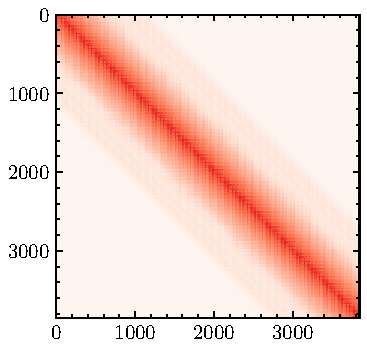
\includegraphics[scale=1.0]{Pics/densityO}
\end{subfigure}
$\Longrightarrow$
\begin{subfigure}{0.4\linewidth}
\centering
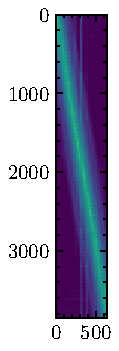
\includegraphics[scale=1.0]{Pics/choleskyO}
\end{subfigure}%
\hfill
\centering
\begin{subfigure}{0.5\linewidth}
\centering
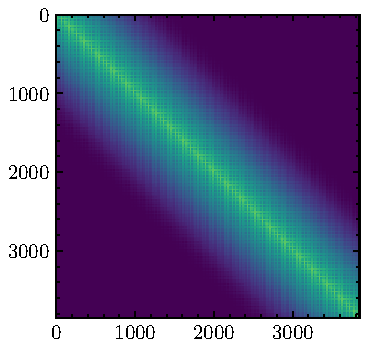
\includegraphics[scale=1.0]{Pics/densityV}
\end{subfigure}
$\Longrightarrow$
\begin{subfigure}{0.4\linewidth}
\centering
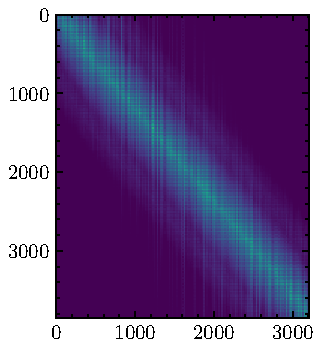
\includegraphics[scale=1.0]{Pics/choleskyV}
\end{subfigure}%
\caption[Cholesky decomposition of density matrices]{Cholesky decomposition, the occupied and virtual density matrices (left) yields a set of coefficients that describe a localized MO basis in the orbital and virtual space, respectively (right). The matrices are represented in terms of a heat map which indicates the magnitude of $log_{10}(abs(a_{ij}))$.}
\label{fig:LOCORB_CHOL}
\end{figure} 

\subsection{Natural Orbitals}

While the schemes described above try to generate a set of occupied and/or virtual molecular orbitals localized in space, natural orbital (NOs) methods try to generate a set of "compact" orbitals, i.e. a minimal set of orbitals that can describe the problem at hand. The concept of natural orbitals was first introduced by Löwdin \cite{Low1956}. The natural orbitals $\Theta_i$ of a wave function $\Psi$ are defined as the eigenfunctions of the one-particle density operator $\hat{n}$

\begin{equation}
\hat{n}\ket{\Theta_i} = n_i \ket{\Theta_i} 
\end{equation}

\noindent where $n_i$ are the occupation numbers of the associated orbital $\Theta_i$. One can then choose a reduced orbital space $\{\tilde{\Psi}_i\}$ by only taking into account those orbitals with an occupation number above a certain threshold $\tau$. The orbitals are "natural" in the sense that they are determined purely using $\Psi$, and are intrinsic to the system. NOs are computed by diagonalizing the one-particle density matrix at the desired level of theory (Hartree-Fock, MP, CIS, CC). 

%NOs are state-specific (Pok2019), meaning that NOs computed from the ground state densities may not be well suited to describe excited states, and NOs of different excited states might also greatly differ. As such, as will be later shown for local flavours of ADC, NOs need to be recomputed for each state.

% CIS(D) density matrices https://aip.scitation.org/doi/pdf/10.1063/1.4983277

\subsubsection{Natural Orbitals in Hartree Fock Theory}

In Hartree Fock theory, natural orbitals are mostly reserved for qualitative population and bond order analysis. 

Natural atomic orbitals (NAOs) are computed by diagonalizing the blocks $P_{\mu_A\nu_A}$ of the atomic density matrix, where ${\mu_A}$, ${\nu_A}$ are basis functions centered on atom $A$. NAOs are optimal for describing the electron density around individual atom centers. NAOs are also useful for obtaining a set of guess orbitals from density matrices formed from the superposition of atomic densities (SAD) guess (Annex \ref{app:SCFGUESS}). 

Furthermore, NAOs serve as the starting point for obtaining natural hybrid orbitals (NHOs), which in turn are used for constructing natural bond orbitals (NBOs). NBOs are a useful orbital representation for  analyzing molecular bonds (e.g. bond order, bond polarity). They are conceptually close to the traditional Lewis structure of a molecule \cite{Ree1983,Wei2001,Gle2012}.

% (ref: https://pubs.acs.org/doi/pdf/10.1021/ja00544a007)
% NBOs https://aip.scitation.org/doi/pdf/10.1063/1.445134
% NAOs, NBOs https://pubs.rsc.org/en/content/articlepdf/2001/rp/b1rp90011k
% (Recent) NBOs https://onlinelibrary.wiley.com/doi/epdf/10.1002/wcms.51
% https://goldbook.iupac.org/terms/view/NT07076

\subsubsection{Frozen Natural Orbitals}

For large basis sets, the number of occupied canonical MOs is several times lower than the number of virtual canonical orbitals. Furthermore, NOs do not considerably reduce the number of occupied orbitals. It is therefore sufficient to only compute the eigenfunctions of the virtual-virtual block of the one-particle density matrix, in what is known as the frozen natural orbitals (FNOs) approach \cite{Bar1970}. FNOs need information of the correlated wave function, and are therefore typically computed at a lower level of theory. For example, the easiest way to obtain a set of FNOs for CCSD or CCSD(T) computation is to diagonalize the virtual-virtual block  of the MP2 density matrix \cite{Sos1989, Tau2005, Tau2008}
\begin{equation}
D_{ab} = \frac{1}{2} sum_{cij} \frac{K_{ij}^{cb} K_{ij}^{ca}}{\eps_{ij}^{ab} \eps_{ij}^{ca}}
\end{equation}
\noindent with
\begin{equation}
K_{ij}^{ab} = 2 \cn{ia}{jb} - \cn{ib}{ja}
\end{equation}
\begin{equation}
\eps_{ij}^{ab} = \eps_i + \eps_j - \eps_a - \eps_b 
\end{equation}
The FNOs are then canonicalized (\ref{app:CANON}). The combined set of occupied CMOs and virtual FNOs forms a very compact representation suitable for CC ground state and excited state calculations.

% MP2 NOs:
% Jor1988 J. Chem. Phys. 88, 3834 (1988); https://doi.org/10.1063/1.453884
% D. M. Silver and R. J. Bartlett,Phys. Rev. A13,1 1976.
% D. M. Silver, S. Wilson, and R. J. Bartlett,Phys. Rev. A16,477 1977.

% FNOs: 
% Bar1970 Phys. Rev. A 1, 644 – Published 1 March 1970

% FNO CC: 
% Sos1989 https://doi.org/10.1016/0009-2614(89)87399-3
% Tau2005 Taube, Andrew G.; Bartlett, Rodney J. (2005). Frozen Natural Orbitals: Systematic Basis Set Truncation for Coupled-Cluster Theory. Collection of Czechoslovak Chemical Communications, 70(6), 837–850. doi:10.1135/cccc20050837  
% A. G. Taube and R. J. Bartlett,  Frozen natural orbital coupled-cluster theory:  Forces andapplication to decomposition of nitroethane,  J. Chem. Phys.128, 164101 (2008)
% CCLR NO  A. Kumar and T. D. Crawford,   Frozen virtual natural orbitals for coupled-cluster linear-response theory,  J. Phys. Chem. A121, 708 (2017).

% Have a look at Pok2019 https://chemrxiv.org/articles/preprint/Extension_of_Frozen_Natural_Orbital_Approximation_to_Open-Shell_References_Theory_Implementation_and_Application_to_Single-Molecule_Magnets/10308053/1

\subsubsection{Natural Transition Orbitals}

Consider the CIS eigenvalue problem for finding the excitation energies $\omega_n$ and their associated transition density matrices $R_n$

\begin{equation}
\mathbf{A_{CIS}} R_n = \omega_n R_n 
\end{equation}

The matrices $\mathbf{R}_n$ contain $n_{occ}n_{vir}$ expansion coefficients $c_{ia}$ which show how much an orbital-virtual MO pair $ia$ contributes to the excitation $n$. The number of non-negligible coefficients can be far from zero, making interpretations of the computed results difficult for some systems.

Natural transition orbitals (NTOs) were introduced to facilitate the qualitative description of an excited state and finding connections to experimental spectra \cite{Luz1976, Mar2003}. NTOs are typically obtained by computing the singular value decomposition (SVD) of the state densities $\mathbf{R}_n$

\begin{equation}
\mathbf{R} = \mathbf{U} \mathbf{\Sigma} \mathbf{V}^{\dagger}  
\end{equation} 

\noindent where $\mathbf{U}$ and $\mathbf{V}$ are unitary matrices with dimension $n_{occ} n_{NTO}$ and $n_{vir}n_{NTO}$, and $\Sigma$ is a $n_{NTO}$ by $n_{NTO}$ matrix containing the singular values $s$ on its diagonal. The CMOs $\{\Psi^{occ}_i,\Psi^{vir}_a\}$ are transformed to the NTO basis $\{\overline{\Psi}^{occ}_k,\overline{\Psi}^{vir}_k\}$ using

\begin{equation}
\ket{\overline{\Psi}^{occ}_k} = U_{ki} \ket{\Psi^{occ}_i}
\end{equation}
\begin{equation}
\ket{\overline{\Psi}^{vir}_k} = V_{ka} \ket{\Psi^{vir}_a}
\end{equation}

\noindent The singular value $s_k$ show the contribution of an NTO pair $k$ to the excited state. In most cases, the number of significant NTO pairs is significantly lower than $n_{occ}n_{vir}$ and at most equal to $n_{occ}$. NTOs are not limited to CIS, but can also be obtained by SVD decomposition of the singles-singles block of excited state densities from higher order methods such as ADC or CCLR. 

Natural transition orbitals have also found use in local excited  state correlation methods \cite{Bau2017,Hof2017}, where CIS NTOs are combined with MP2 NOs to obtain a compact orbital representation for ground and excited state coupled cluster calculations.

EXAMPLE!!! phenylalanine

% Luz1976 https://link.springer.com/article/10.1007%2FBF00526670

% Mar2003 https://aip.scitation.org/doi/pdf/10.1063/1.1558471

% https://www.sciencedirect.com/science/article/pii/S0009261407002072?via%3Dihub

% CornFlex: Bau2017 https://aip.scitation.org/doi/pdf/10.1063/1.4984820

% Hof2017 Natural transition orbitals for the calculation of correlation andexcitation energies

\subsection{Specific Virtual Orbitals}

In most cases, using LMOs instead of CMOs does not offer any a priori advantage in terms of the computational complexity associated with correlated methods, and additional approximations are necessary. In local correlation methods, this is often done by truncating the VMO space. Truncation of the VMOs has been an active field of research for several decades. A naive approach to truncate the virtual space would be to eliminate VMOs with orbital energies above a certain threshold; however, this proved to be unusable in most contexts \cite{Sen2011}. More successful methods for VMO truncation use the concept of what will referred to as \emph{specific virtual orbitals} (SVOs). SVOs are specific in the sense that each individual occupied MO $i$ or each pair of MOs $ij$ has their own set of SVOs $a_i$ (orbital specific virtual orbitals) or a$_{ij}$ (pair specific virtual orbitals) associated to it.
The concept of SVOs naturally arises in the context of correlated methods such as the coupled electron pair approximation (CEPA) where the total energy is computed is computed as the sum of electron pair energies $e$
\begin{equation}
E_{CEPA} = \sum_{ij} e_{ij}
\end{equation}
The electron pair energy decays rapidly as a function of the distance $r$ between MO centers in an LMO basis. Distant virtual orbitals contribute less to the electron pair energy as virtual orbitals close to ${ij}$. It has been shown early on that instead of using the whole virtual orbital span, one can correlate only a subset or reduced set of virtual orbitals with each electron pair \cite{Sae1985,Edm1965,Mey1971,Mey1973}
%(0,1,2,3) 
and still recover most of the correlation energy. In the limit of large molecules, the number of significant virtual orbitals for an electron pair becomes independent of system size \cite{Kra2012} (see also Chapter 4). There are different ways to choose how to define the VMO subsets, either by using local molecular orbitals or natural orbitals.

% 0 BASIS FOR LMO-PAO S. Saebø and P. Pulay , Chem. Phys. Lett., 1985, 113 , 13
% 1 BASIS FOR PNOs Edmiston, C.; Krauss, M. Configuration-interaction calculation of H3 and H2. J. Chem. Phys. 1965, 42, 1119– 1120,  DOI: 10.1063/1.1696050 
% 2 OTHER Meyer, W. Ionization energies of water from PNO-CI calculations. Int. J. Quantum Chem. 1971, 5, 341– 348,  DOI: 10.1002/qua.560050839 
% 3 ALSO Meyer, W. PNO-CI Studies of electron correlation effects. I. Configuration expansion by means of nonorthogonal orbitals, and application to the ground state and ionized states of methane. J. Chem. Phys. 1973, 58, 1017– 1035,  DOI: 10.1063/1.1679283
% 4 https://pubs.rsc.org/am/content/articlehtml/2012/cp/c2cp40231a#cit51

\subsubsection*{Domain Specific Virtual Orbitals}

The term \emph{domain specific virtual orbitals} (DSVOs) will be used to denote any type of virtual orbitals where the subsets are formed \emph{a priori} by distance or partial charge criteria. Examples include the local MP2 and local CCSD implementations by Schütz et al. \cite{Sch1999,Sch2001,Sch2000}.%(AA,AB,AC)

First, occupied CMOs are localized by one of the methods described above, e.g. FB or ER. Virtual CMOs are transformed into the PAO basis. Each individual occupied LMO $\ket{\Psi_i}$ is then assigned a subset $[i]$ of PAOs, chosen by a Boughton-Pulay (BP) criterion \cite{Bou1993} or by population analysis \cite{Mat2008}. 

For a given electron pair $ij$, the pair domain is then formed by taking the union $[ij]$ = $[i] \cup [j]$. The set of all virtual pair domains $[ij]$ forms the DSVOs.

Alongside AOs, DSVOs were among the first orbital representations in which linear scaling correlated methods were formulated. Their dependency on distance criteria for selecting the pair domains makes them less rigorous than other methods, and they have fallen out of favor over the years.

% Local LMO-PAO
% AA M. Schütz , G. Hetzer and H.-J. Werner , J. Chem. Phys., 1999, 111 , 5691
% AB M. Schütz and H.-J. Werner , J. Chem. Phys., 2001, 114 , 661
% AC M. Schütz and H.-J. Werner , Chem. Phys. Lett., 2000, 318 , 370 
% AD https://onlinelibrary.wiley.com/doi/abs/10.1002/jcc.540140615
% AE R. A. Mata, H.-J. Werner, S. Thiel and W. Thiel, J. Chem. Phys., 2008, 128, 025104

\subsubsection*{Pair Natural Orbitals}
% Review: https://pubs.rsc.org/am/content/articlehtml/2012/cp/c2cp40231a
First introduced under the guise of "pseudo-natural orbitals" \cite{Edm1965}, then rediscovered by Neese \cite{Nee2009a,Nee2009b,Han2011}, projected natural orbitals (PNOs) have risen in popularity in the recent years. Similarly to DSVMOs, each electron pair has a set of PNOs associated to it. PNOs are formed by diagonalizing the MP2 pair density matrix for each MO pair $ij$ (hence "pair-natural")

\begin{equation}
\mathbf{D}^{ij} = \frac{1}{1+\delta_{ij}} \left(\tilde{\mathbf{t}}^{ij} \mathbf{t}^{ij} + tilde{\mathbf{t}}^{ij} \mathbf{t}^{ij\dagger} \right)
\end{equation}

\noindent with 

\begin{equation}
\mathbf{\tilde{t}}^{ij}_{ab} = 2 \mathbf{t}^{ij}_{ab} - \mathbf{t}^{ji}_{ab} 
\end{equation}

\noindent The eigenvalue decomposition of $\mathbf{D}$ then gives

\begin{equation}
\mathbf{D}^{ij} \mathbf{Q}^{ij} = n^{ij} \mathbf{Q}^{ij} 
\end{equation}

\noindent where $\mathbf{Q^{ij}}$ are the pair specific transformation matrices, and $n^{ij}$ their occupation numbers. The Fock matrix in the LMO representation is not diagonal, and the MP2 amplitudes are approximated by

\begin{equation}
t_{ij}^{ab} = \frac{\cn{ia}{jb}}{\eps_a + \eps_b - f_{ii} - f_{jj}}
\end{equation}

\noindent where $f_{ii}$ are the diagonal entries of the Fock matrix in the LMO basis. The pair domains $[ij]$ are chosen by keeping the PNOs with an occupation number larger than a threshold $\tau_{PAO}$. Therefore, accuracy is controlled by a single, distance-independent parameter, which is an advantage over other methods like DSVOs. 

However, computing the PNOs requires a full MP2 calculation, and with density fitting scales with $\ccpx{5}$. Moreover, even if the PNO basis is compact, the fact that each LMO pair has its own virtual orbital basis may lead to a prohibitively large number of PNOs for large molecules.

The concept of PNOs can be combined with the domain-based approach using LMOs, in what is known as local pair-natural orbitals (LPNOs) \cite{Rip2013}. 

% CA F. Neese, F. Wennmohs and A. Hansen, J. Chem. Phys., 2009, 130, 114108 CrossRef .
% CB F. Neese, A. Hansen and D. G. Liakos, J. Chem. Phys., 2009, 131, 064103 CrossRef .
% CC A. Hansen, D. G. Liakos and F. Neese, 2011, 135, 214102.

%Local PNOs:
% https://aip.scitation.org/doi/10.1063/1.4773581

\subsubsection*{Orbital Specific Virtuals}

Closely related to PNOs are the orbital specific virtual orbitals (OSVs) \cite{Yan2011}. The OSVs for an LMO $\ket{\Psi_i}$ are obtained by taking the diagonal PNOs for the domain $[ii]$. The MP2 density matrix reduces to

\begin{equation}
\mathbf{D}^{ii} = 4 \mathbf{t}^{ii} \mathbf{t_{ii}}
\end{equation}

Instead of reducing the density matrix, one can just diagonalize $\mathbf{t}^{ij}$ instead. 

\begin{equation}
\mathbf{t}^{ii} \mathbf{Q}^{ii} = t^{ii} \mathbf{Q}^{ii}
\end{equation}

\noindent where $t^{ii}$ are the eigenvalues, which are used to compute the compute the occupation numbers $n^{ii} = \left( t^{ii} \right)^2$. OSVs for which $n^{ii} > \tau_{OSV}$ are included into the orbital specific domain $[i]$. Pair domains $[ij]$ are then formed as the union of $[i]$ and $[j]$ similar to DSVOs. 

OSVs have the advantage that the can be constructed with $\ccpx{3}$ scaling provided that density fitting is used. However, OSVs are less compact than PNOs.

OSVs can be used to lower the computational complexity to construct PNOs. Several hybrid OSV-PNO schemes have been proposed with a computational complexity of $\ccpx{4}$ \cite{Kra2012}, $\ccpx{3}$ \cite{Sch2013} and finally $\mathcal{O}(N)$ \cite{Rip2013}.

%\subsubsection{Local Pair Natural Orbitals}

% Rip2013 https://aip.scitation.org/doi/pdf/10.1063/1.4773581

%NAFs: \url{https://aip.scitation.org/doi/full/10.1063/1.4905005}
% DLPNO: relationship between i and X https://aip.scitation.org/doi/pdf/10.1063/1.4926879

